% !TEX root = ./main.tex
% !TEX encoding = UTF-8 Unicode
\documentclass[a4paper,12pt]{article}

% ==================================================
% Sprache und Zeichencodierung
\usepackage[german]{babel}
\usepackage[utf8]{inputenc}
\usepackage[T1]{fontenc}

% ==================================================
% Seitenlayout
\usepackage[
  left=2.5cm,
  right=2.5cm,
  top=2.5cm,
  bottom=2.5cm
]{geometry}

% ==================================================
% Mathematik
\usepackage{amsmath}
\usepackage{amsfonts}
\usepackage{amssymb}
\usepackage{amsthm}
\usepackage{physics}
\usepackage{mathrsfs}
\usepackage{dsfont}
\usepackage{esint}

% ==================================================
% Programmierung
\usepackage{listings}

% ==================================================
% Textgestaltung
\usepackage{enumerate}
\usepackage[shortlabels]{enumitem}
\usepackage{framed}
\usepackage{csquotes} % wichtig für deutsche Anführungszeichen
\usepackage{microtype} % bessere Silbentrennung und Schriftbild

% ==================================================
% Tabellen, Grafiken
\usepackage{float}
\usepackage{tabularx}
\usepackage{multicol}
\usepackage{caption}
\usepackage{subcaption}
\captionsetup{
    format=hang,
    margin=10pt,
    font=small,
    labelfont=bf
}

% ==================================================
% Literaturverzeichnis
\usepackage[
    backend=biber,
    style=authoryear,
    natbib=true
]{biblatex}
\addbibresource{literatur.bib}

% ==================================================
% Hyperlinks
\usepackage{hyperref}
\usepackage{xcolor}
\definecolor{links}{rgb}{0.36,0.54,0.66}
\hypersetup{
    colorlinks=true,
    linkcolor=black,
    urlcolor=links,
    citecolor=links,
    filecolor=links,
    pdfauthor={Dein Name},
    pdftitle={Titel der Arbeit},
    pdfsubject={Hausarbeit},
    pdfkeywords={Schlüsselwort1, Schlüsselwort2},
    pdfproducer={LaTeX},
    pdfcreator={pdfLaTeX}
}

% ==================================================
% Eigene Befehle (optional)
\newcommand{\R}{\mathbb{R}} % Beispiel für eigene Makros

\usepackage{titlesec}
\usepackage[many]{tcolorbox}

% Adjust spacing after the chapter title
\titlespacing*{\chapter}{0cm}{-2.0cm}{0.50cm}
\titlespacing*{\section}{0cm}{0.50cm}{0.25cm}

% Indent 
\setlength{\parindent}{0pt}
\setlength{\parskip}{1ex}

% --- Theorems, lemma, corollary, postulate, definition ---
% \numberwithin{equation}{section}

\newtcolorbox{problem}[1][]{
    enhanced,
    colback = black!5,
    colbacktitle = black!5,
    coltitle = black,
    boxrule = 0pt,
    frame hidden,
    borderline west = {0.5mm}{0.0mm}{black},
    fonttitle = \bfseries\sffamily,
    breakable,
    before skip = 3ex,
    after skip = 3ex,
    sharp corners,
    fontupper = \raggedright,
    #1
}


\tcbuselibrary{skins, breakable}

% --- You can define your own color box. Just copy the previous \newtcbtheorm definition and use the colors of yout liking and the title you want to use.
% --- Basic commands ---
% Farben definieren
\definecolor{codegreen}{rgb}{0,0.6,0}
\definecolor{codegray}{rgb}{0.5,0.5,0.5}
\definecolor{codepurple}{rgb}{0.58,0,0.82}
\definecolor{backcolour}{rgb}{0.95,0.95,0.92}

%   Euler's constant
\newcommand{\eu}{\mathrm{e}}

%   Imaginary unit
\newcommand{\im}{\mathrm{i}}

%   Sexagesimal degree symbol
\newcommand{\grado}{\,^{\circ}}

% --- Inline C++ Code mit Syntax-Highlighting ---

% Listings-Style für C++
\lstdefinestyle{cppstyle}{
    language=C++,
    basicstyle=\ttfamily\small,
    keywordstyle=\color{blue},
    stringstyle=\color{codepurple},
    commentstyle=\color{codegreen},
    morecomment=[l][\color{magenta}]{\#},
    backgroundcolor=\color{backcolour},
    breaklines=true,
    breakatwhitespace=true,
    columns=fullflexible
}

% Inline C++ Command
\newcommand{\cppinline}[1]{\lstinline[style=cppstyle]{#1}}


% --- Comandos para álgebra lineal ---
% Matrix transpose
\newcommand{\transpose}[1]{{#1}^{\mathsf{T}}}

%%% Comandos para cálculo
%   Definite integral from -\infty to +\infty
\newcommand{\Int}{\int\limits_{-\infty}^{\infty}}

%   Indefinite integral
\newcommand{\rint}[2]{\int{#1}\dd{#2}}

%  Definite integral
\newcommand{\Rint}[4]{\int\limits_{#1}^{#2}{#3}\dd{#4}}

%   Dot product symbol (use the command \bigcdot)
\makeatletter
\newcommand*\bigcdot{\mathpalette\bigcdot@{.5}}
\newcommand*\bigcdot@[2]{\mathbin{\vcenter{\hbox{\scalebox{#2}{$\m@th#1\bullet$}}}}}
\makeatother

%   Hamiltonian
\newcommand{\Ham}{\hat{\mathcal{H}}}

%   Trace
\renewcommand{\Tr}{\mathrm{Tr}}

% Christoffel symbol of the second kind
\newcommand{\christoffelsecond}[4]{\dfrac{1}{2}g^{#3 #4}(\partial_{#1} g_{#2 #4} + \partial_{#2} g_{#1 #4} - \partial_{#4} g_{#1 #2})}

% Riemann curvature tensor
\newcommand{\riemanncurvature}[5]{\partial_{#3} \Gamma_{#4 #2}^{#1} - \partial_{#4} \Gamma_{#3 #2}^{#1} + \Gamma_{#3 #5}^{#1} \Gamma_{#4 #2}^{#5} - \Gamma_{#4 #5}^{#1} \Gamma_{#3 #2}^{#5}}

% Covariant Riemann curvature tensor
\newcommand{\covariantriemanncurvature}[5]{g_{#1 #5} R^{#5}{}_{#2 #3 #4}}

% Ricci tensor
\newcommand{\riccitensor}[5]{g_{#1 #5} R^{#5}{}_{#2 #3 #4}}

\begin{document}

\begin{Large}
    \textsf{\textbf{CPU Algorithm Design}} \\
    \\
    Exercise 3
\end{Large}
\vspace{1ex}
\textsf{\textbf{Students:}} \text{Vishal Mangukiya, Konstantin Benz} \\
\vspace{2ex}

\section*{3.1 Adapting reduce and transform}

The input containers in \cppinline{reduce\_LoopUnrolling\_view.hpp} and \\
\cppinline{transform\_LoopUnrolling\_view.hpp} were adapted to use range-based views as requested in the assignment. \\
In the reduction routines, the memory-backed containers were replaced with \cppinline{std::views::repeat(1.0f, N)},
using \cppinline{decltype(std::views::repeat(...))} to define a compatible member variable. This makes the code compute-bound and avoids unnecessary memory usage. \\
For the transform routines, the input values were changed to \cppinline{std::ranges::views::iota(0, N)}. Additionally, the output container \cppinline{W} was replaced by a fixed-size \cppinline{std::vector<Real>(256)} with modulo-indexed access to enable reuse of the output buffer and simulate non-memory-bound processing.

\textbf{Challenges encountered:}
\begin{itemize}
    \item Initially, the range variables \cppinline{V} and \cppinline{W} were only declared inside each function. However, since multiple functions need access to them, we had to promote them to class-level member variables.
    \item Using \cppinline{std::views::repeat} or \texttt{std::views::iota} as class members required careful type declarations. Simple type aliases like \cppinline{std::ranges::repeat\_view} or \cppinline{std::ranges::iota\_view} caused type mismatch errors when assigning views with bounds.
    \item The correct approach was to use \cppinline{decltype(std::views::repeat(...))} and \\
          \cppinline{decltype(std::views::iota(...))} for the member declarations, as this ensured compatibility with the generated view types and compiler support on the cluster (GCC 14).
    \item Some loops were not vectorized according to compiler warnings. Since manual unrolling was explicitly requested in the assignment, we did not attempt further refactoring in these cases.
\end{itemize}

All modified functions were compiled and tested successfully via the targets \\
\texttt{reduceVbenchmarkUnroll} and \texttt{transformVbenchmarkUnroll}.

\pagebreak

\section*{3.2 Adapting benchTransformUnrollLoopPeelingDirective}

The function \cppinline{benchTransformUnrollLoopPeelingDirective} was implemented using \\
\cppinline{std::views::iota} for input generation and a fixed-size \cppinline{std::vector} with modulo indexing for the output buffer.
The loop is unrolled using the custom \cppinline{UNROLLFACTOR} macro and processes SIMD batches via \cppinline{xsimd::batch}.
We ensured compatibility by using \cppinline{static\_assert(unroll\_factor \% simd\_width == 0)} and unaligned load/store operations for safe access to the input and output.

We used \texttt{unrollScript.sh} to benchmark the function for various unroll factors. The results are stored in the \texttt{changingUnrollFactor/res/} directory on the cluster and in \\
the \texttt{benchmark} folder in the submitted archive and will be analyzed in section 3.5.

\pagebreak

\section*{3.3 Adapting benchReduceUnrollTreeDirective}

The function \cppinline{benchReduceUnrollTreeDirective} was implemented using a recursive tree-reduction strategy with a configurable tree degree.
The reduction starts with a \\
\cppinline{std::array<Real, unroll\_factor>} which is filled from the \cppinline{std::views::repeat} input.

A loop successively reduces this array in-place using groups of \cppinline{tree\_deg} elements per node.
This process continues as long as the array size is divisible by \cppinline{tree\_deg}.
If a remainder is left (i.e. fewer than \cppinline{tree\_deg} values remain), a final sequential sum is performed.

This design ensures flexibility for various unroll and tree degrees. We used \\
\cppinline{static\_assert(unroll\_factor \% tree\_deg == 0)} to catch invalid configurations at compile time.
The remainder of the input (\cppinline{N \% unroll\_factor}) is processed separately via a scalar OpenMP loop.

The implementation successfully compiles and runs within the benchmark target \\
\cppinline{reduceVbenchmarkUnroll}.

\pagebreak

\section*{3.4 Adapting benchReduceUnrollSimdXHorizontal and benchReduceUnrollSimdXVertical}

\subsection*{Horizontal}

The function \cppinline{benchReduceUnrollSimdXHorizontal} performs a flat reduction of all elements within an \cppinline{unroll\_factor}-sized block.
Each SIMD batch of \cppinline{simd\_width} elements is summed and accumulated into a single SIMD register, which is then reduced to scalar using \cppinline{xsimd::reduce\_add}.

\subsection*{Vertical}

The function \cppinline{benchReduceUnrollSimdXVertical} uses a tree-like structure of SIMD lanes.
It maintains \cppinline{unroll\_factor / simd\_width} SIMD accumulators, one for each logical reduction path.
Input vectors are dispatched into different SIMD accumulators in parallel. The final scalar result is obtained by reducing all lanes individually.

\pagebreak

\section*{3.5 Benchmarking and Performance Analysis}

\subsection*{Reduce Benchmarks}

Figure~\ref{fig:reduce} shows the average execution time of all reduce benchmark variants.

\begin{figure}[h]
    \centering
    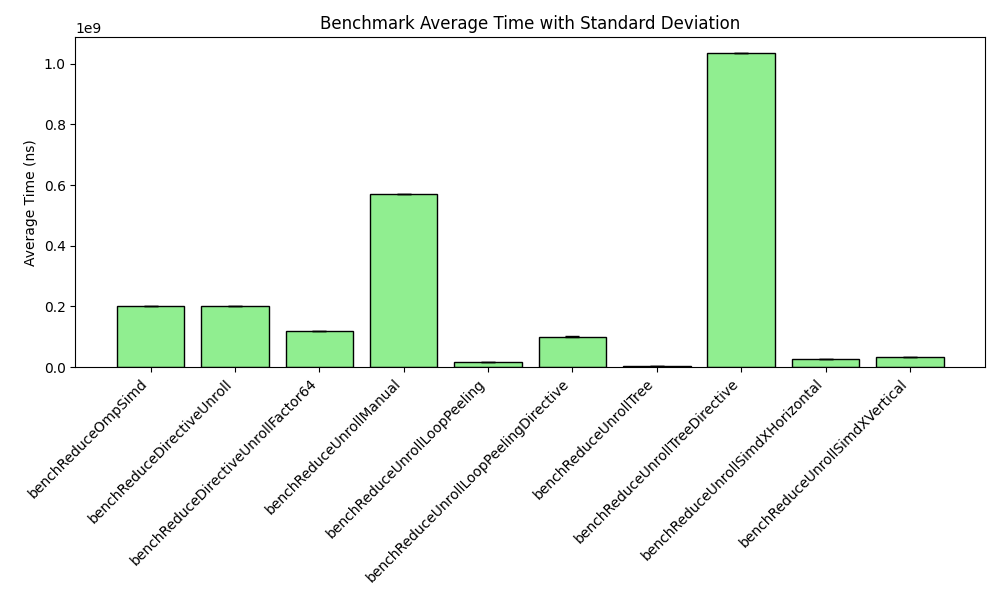
\includegraphics[width=0.9\textwidth]{img/reduce_results.csv_ex02.png}
    \caption{Reduce variants: average execution time with standard deviation.}
    \label{fig:reduce}
\end{figure}

The results show that:
\begin{itemize}
    \item \cppinline{benchReduceUnrollTree} performs best in terms of runtime. Its logarithmic reduction depth and low overhead make it ideal for large-scale reductions.
    \item \cppinline{benchReduceUnrollManual} performs significantly worse than expected. This is likely due to poor compiler optimization of the 64 manually unrolled assignments without SIMD vectorization.
    \item Surprisingly, \cppinline{benchReduceUnrollSimdXHorizontal} performs \emph{worse} than all others. This may be due to register spilling or poor instruction scheduling on our test hardware.
    \item The best trade-off between performance and implementation effort is found in \cppinline{benchReduceUnrollTreeDirective}, though it is still slower than the plain \cppinline{...Tree} version.
\end{itemize}

\subsection*{Transform Benchmarks}

Figure~\ref{fig:transform} shows the average execution time of all transform variants.

\begin{figure}[h]
    \centering
    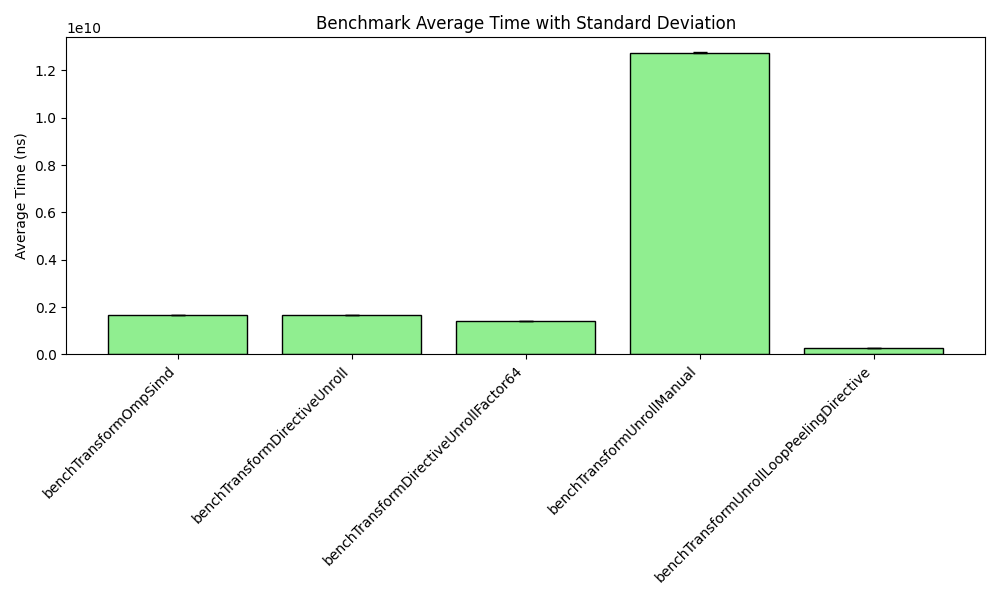
\includegraphics[width=0.9\textwidth]{img/transform_results.csv_ex02.png}
    \caption{Transform variants: average execution time with standard deviation.}
    \label{fig:transform}
\end{figure}

We observe:
\begin{itemize}
    \item \cppinline{benchTransformUnrollManual} is by far the slowest variant. This confirms that the compiler cannot effectively vectorize the hand-unrolled code without specific SIMD intrinsics or pragma hints.
    \item \cppinline{benchTransformUnrollLoopPeelingDirective} outperforms all others. This confirms the performance benefit of vectorized unroll-peeling combined with efficient loop directives and use of XSIMD.
    \item All directive-based unrolling versions perform similarly, with slight improvements at unroll factor 64.
\end{itemize}

\subsection*{Conclusion}

The benchmarking highlights that:
\begin{itemize}
    \item Tree-based reductions scale best for large problem sizes and should be preferred for high-performance compute-bound kernels.
    \item Manual unrolling does not guarantee performance improvements and should be avoided unless paired with SIMD-aware instructions.
    \item XSIMD-based loop peeling with directive unrolling delivers the best transform performance, especially when combined with constant unroll factors and proper modulo-based indexing.
\end{itemize}

Overall, the benchmark confirms that compiler-guided vectorization and algorithmic restructuring (tree reduction, loop peeling) are more effective than naïve hand-unrolling.


\end{document}